%%%%%%%%%%%%%%%%%%%%%%%%%%%%%%%%%%%%%%%%%%%%%%%%%%%%%%%%%%%%%%
\subsection{Применение АР-метода для детектирования сигнала с расширенным спектром}
\label{l:sec3_lpc_dma}

В разделе \ref{ssec:lpc_conclusion} было отмечено, что алгоритм детектирования и оценки параметров
требует значительных вычислительных затрат. В данной работе предлагается способ оптимизации алгоритма,
описанного в разделе \ref{ssec4:lpc_cdma_detect}.

Для перебора фаз ПСП воспользуемся БПФ, в результате получим значения оценки АКФ для каждой фазы ПСП (глава \ref{sec1_fft}).
Схема алгоритма представлена на рисунке \ref{pic:lpc_basic2}. 

\begin{figure}[H]
	\center\scalebox{0.9}{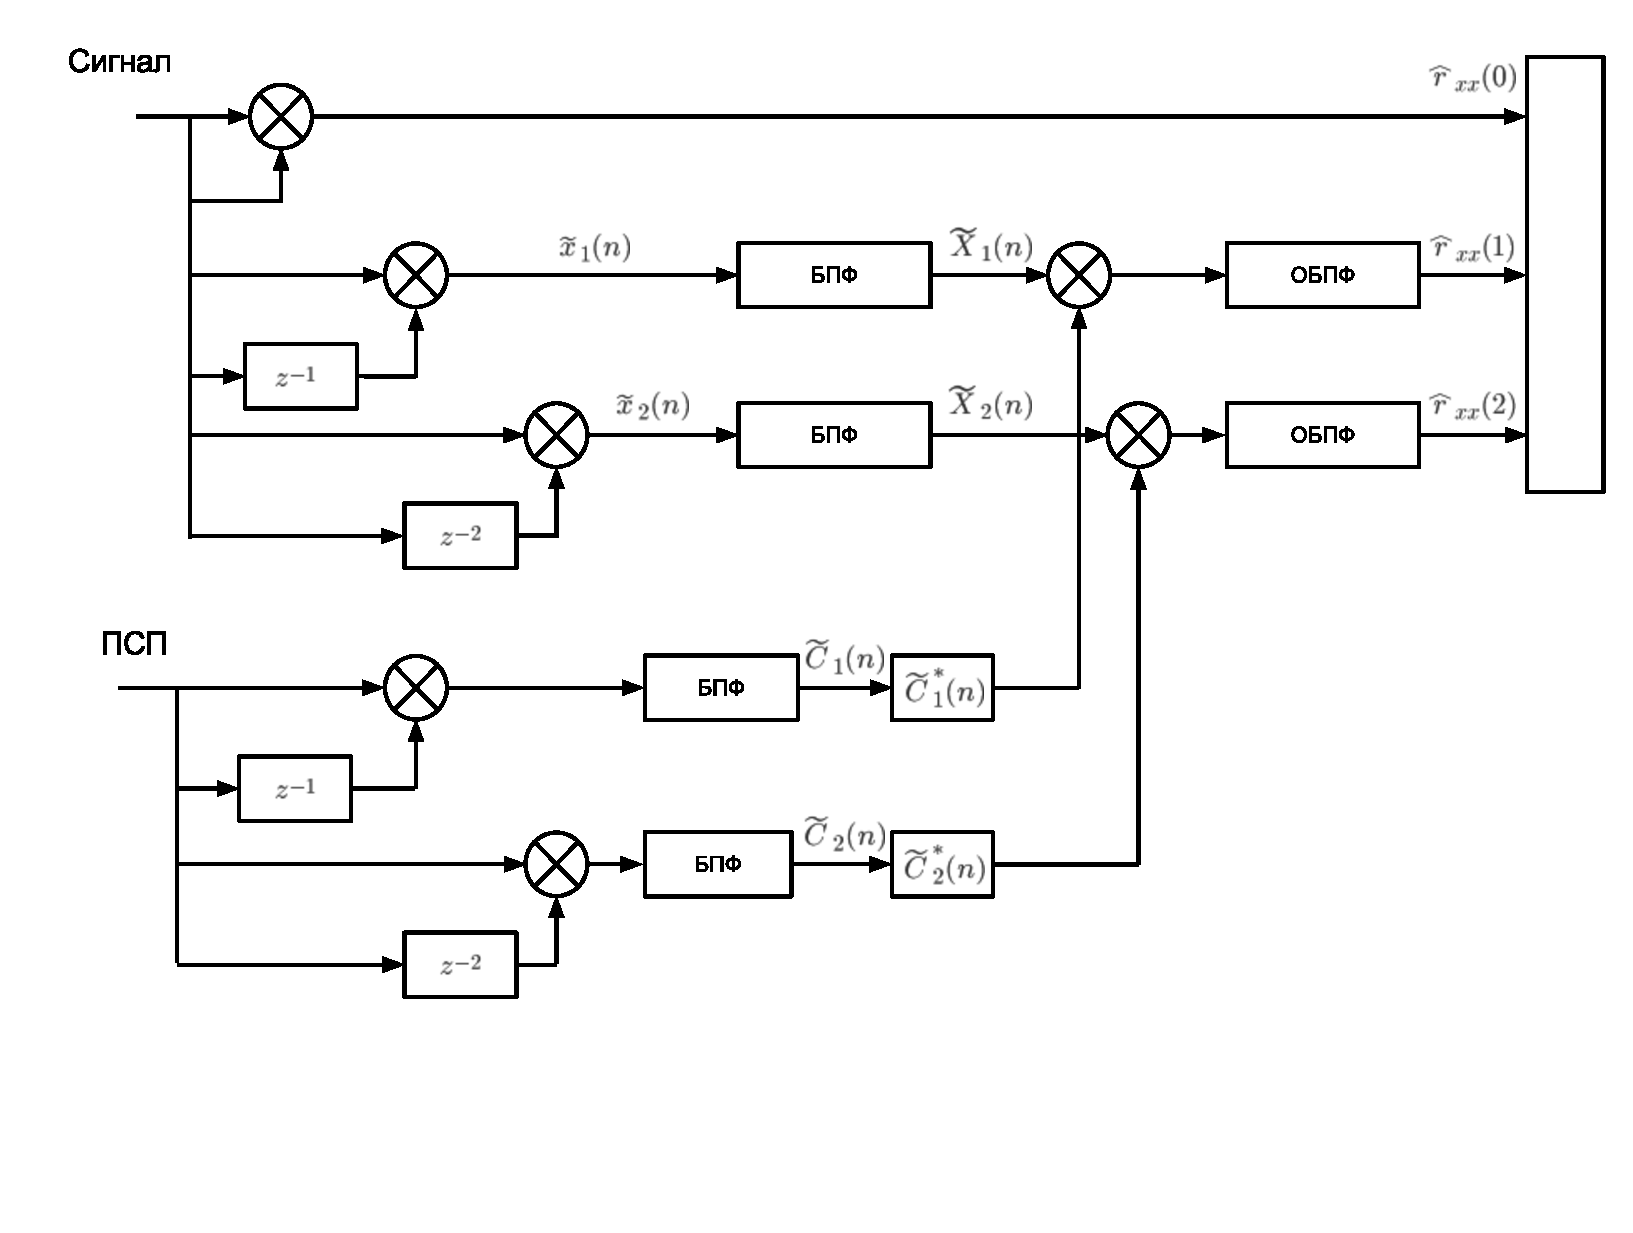
\includegraphics[width=1\linewidth]{lpc_fft.eps}}
	\caption{Схема применения АР-модели для детектирования ШПС сигнала с оптимизацией}
	\label{pic:lpc_basic2}
\end{figure}

Оценка ${\hat{r}_{xx}(0)}$ не зависит от выбранной фазы ПСП, поэтому она вычисляется один
раз для всех смещений кода. Далее формируется массив произведений входного сигнала на
свою задержанную копию ${\tilde{x}_1(n)=x(n)x(n-1)}$. Полученная последовательность  
${\tilde{x}_1(n)}$ поступает на вход алгоритма БПФ, в результате получаем массив ${\tilde{X}_1(n)}$
содержащий частотные отсчеты. Аналогично формируется массив  ${\tilde{X}_2(n)}$ для
задержки входного сигнала равной двум. Таким же способом обрабатываются локально
сгенерированные ПСП и формируются два массива ${\tilde{C}_1(n)}$ и ${\tilde{C}_2(n)}$.
Далее массивы ${\tilde{X}_1(n)}$ и ${\tilde{X}_1(n)}$ поэлементно перемножаются
на комплексно сопряженные массивы ${\tilde{C}_1^*(n)}$ и ${\tilde{C}_2^*(n)}$.
Результаты этих перемножений поступают на вход алгоритма обратного
БПФ. Полученные после ОБПФ два массива содержат оценки автокорреляционной функции для ${N}$ 
смещений кода, где  ${N}$ - размер данных на входе алгоритма БПФ.

Таким образом, предлагаемый алгоритм состоит из следующих шагов:

\begin{itemize}
\item[Шаг 1.] Вычисляются оценки  АКФ в трех первых точках (для аргументов АКФ=0,1,2)
	с использованием алгоритма БПФ для всех возможных смещений ПСП. 
\item[Шаг 2.] Для каждого смещения ПСП: 
	Определяются коэффициенты АР-модели ${\hat{a_1}, \hat{a_2}}$, 
	по формуле \ref{eq:lpc_a_estimation}. 
	Вычисляется резонансная частота ${\omega_0}$
	и определяется квадрат модуля частотного отклика АР-модели для этой частоты. 
\item[Шаг 3.] Выбирается смещение ПСП для которого значение квадрата модуля частотного отклика было максимальным. Полученное значение сравнивается с заранее выбранным порогом детектора. 
	\subitem{\bf{Если}}  значение оказалось больше порогового {\bf{то}} 
		принимается решение о наличии сигнала, а в качестве оценки
		частоты принимается значение ${\omega_0}$ соответствующее выбранному смещению ПСП. 
	\subitem{\bf{Иначе}} 
		Принимается решение об отсутствии гармонического сигнала.
\end{itemize}

%%%%%%%%%%%%%%%%%%%%%%%%%%%%%%%%%%%%%%%%%%%%%%%%%%%%%%%%%%%%%%
\subsection{Подавление интерференции. Алгоритм уточнения оценки АКФ гармонического сигнала.
		Дисперсия оценки АКФ по уточненному алгоритму}
\label{ssec4:quadruple}

Точность АР метода напрямую зависит от тоности оценки АКФ гармонического сигнала. Основным способом повышения точности оценки АКФ является увеличение размера выборки,
что в случае ФМ сигнала может быть затруднительным.В данной работе предлагается использовать алгоритм увеличения ОСШ методом последовательного вычисления
АКФ \cite{ostanin_akf}.

Посчитаем АКФ для выражения \ref{eq:lpc_signal_model2}.

\begin{center}
\begin{equation}
	\label{eq:lpc_akf_n}
	\hat{r}_{xx}(n) = \sum \limits_{k=1}^{K} x(k)x(k+n) = \frac{A^2}{2} \cos{(\omega{n})} \Delta_n \delta{(n)} + \mu{(n)}
\end{equation}
\end{center}

Здесь ${\Delta_n}$ - дисперсия шума ${n(k)}$. ${\mu{(n)}}$ - ошибка оценки АКФ. ${\delta{(n)}}$ - дельта-функция. исперсия ошибки
оценки ${\Delta_{\mu}}$ будет в ${K}$ раз меньше чем дисперсия ${\Delta_n}$ шума в принимаемом сигнале, где ${K}$ - интервал
осреднения оценки АКФ.

Используя оценку АКФ вместо исходной выборки, вновь получим оценку АКФ:
${r_{xx2}(n) = \frac{A^4}{8} \cos{(\omega n)} + \bar{N} \delta{(N)}}$,
где мощность шума оценки ${\bar{N}}$ - будет значительно меньше.

Ампдитуда сигнала на итерации ${k}$ будет равна ${\frac{A^{2^k}}{2^{2^k-1}}}$. Увеличение отношения ОСШ по мощности можно
вычислить по формуле представленной в \cite{book_max}:
\begin{center}
\begin{equation}
	\label{eq:lpc_akf_max}
	G=2BT \frac{1}{2+1/SNR_k}
\end{equation}
\end{center}
где ${G=\frac{SNR_{k+1}}{SNR_k}}$ - относительный прирост ОСШ, ${T}$ - длинна выборки (сек), ${B}$ -  ширина спектра сигнала, 
а ${SNR}$ - ОСШ.

Из \ref{eq:lpc_akf_max} видно, что увеличение ОСШ при вычислении оценки АКФ пропорционально ${2BT}$ и зависит от
ОСШ на входе коррелометра, так же можно отметить, что увеличение ОСШ происходит только при условии ${BT > \frac{1}{2SNR_k} + 1}$.

Так же можно получить оценку АКФ на ${N}$ - шаге. На рисунках \ref{pic:acf_1_iter},
\ref{pic:acf_2_iter}, \ref{pic:acf_3_iter} представлены оценки АКФ на шагах с 1 по 3 для гармонического сигнала при ОСШ -6 дБ.

\begin{figure}[H]
	\center\scalebox{1}{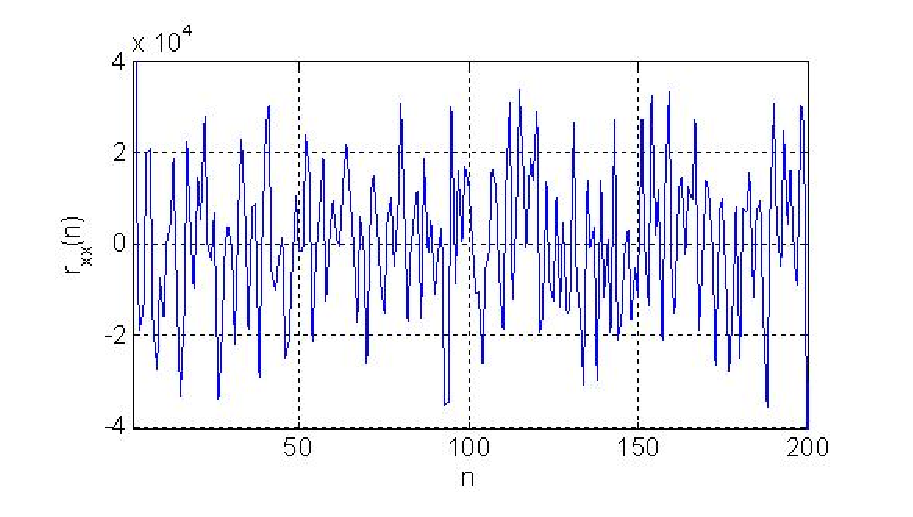
\includegraphics[width=1\linewidth]{acf_1_iter.eps}}
	\caption{Оценка АКФ на 1 итерации.}
	\label{pic:acf_1_iter}
\end{figure}

\begin{figure}[H]
	\center\scalebox{1}{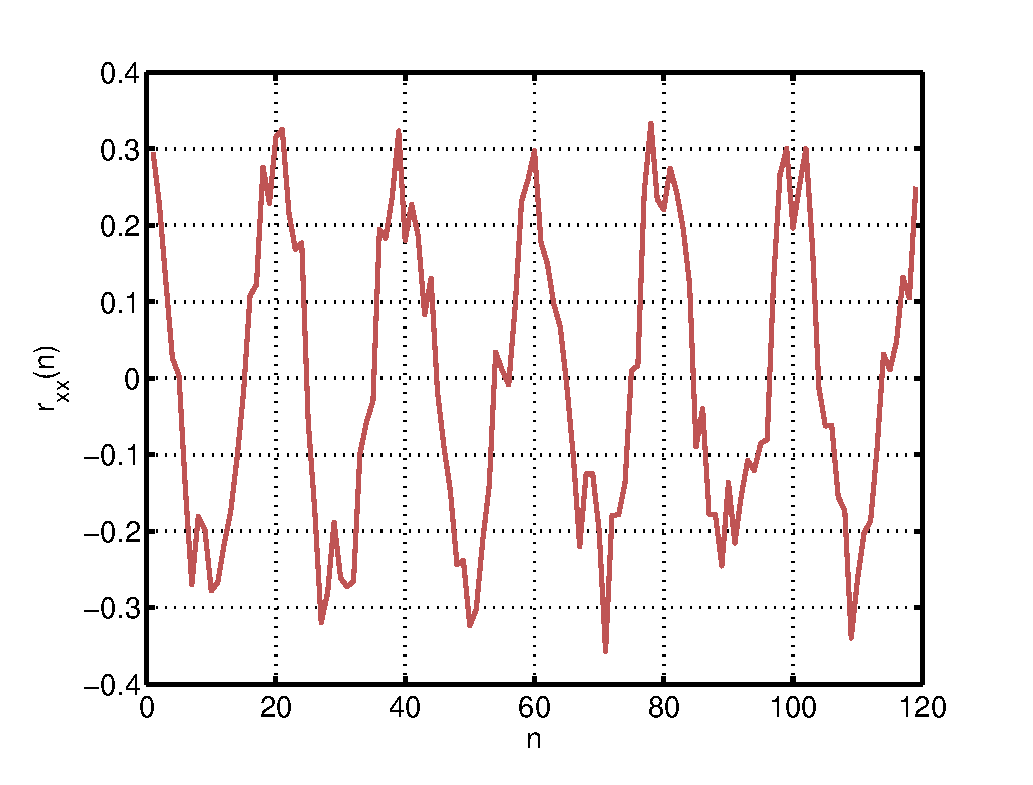
\includegraphics[width=1\linewidth]{acf_2_iter.eps}}
	\caption{Оценка АКФ на 2 итерации.}
	\label{pic:acf_2_iter}
\end{figure}

\begin{figure}[H]
	\center\scalebox{1}{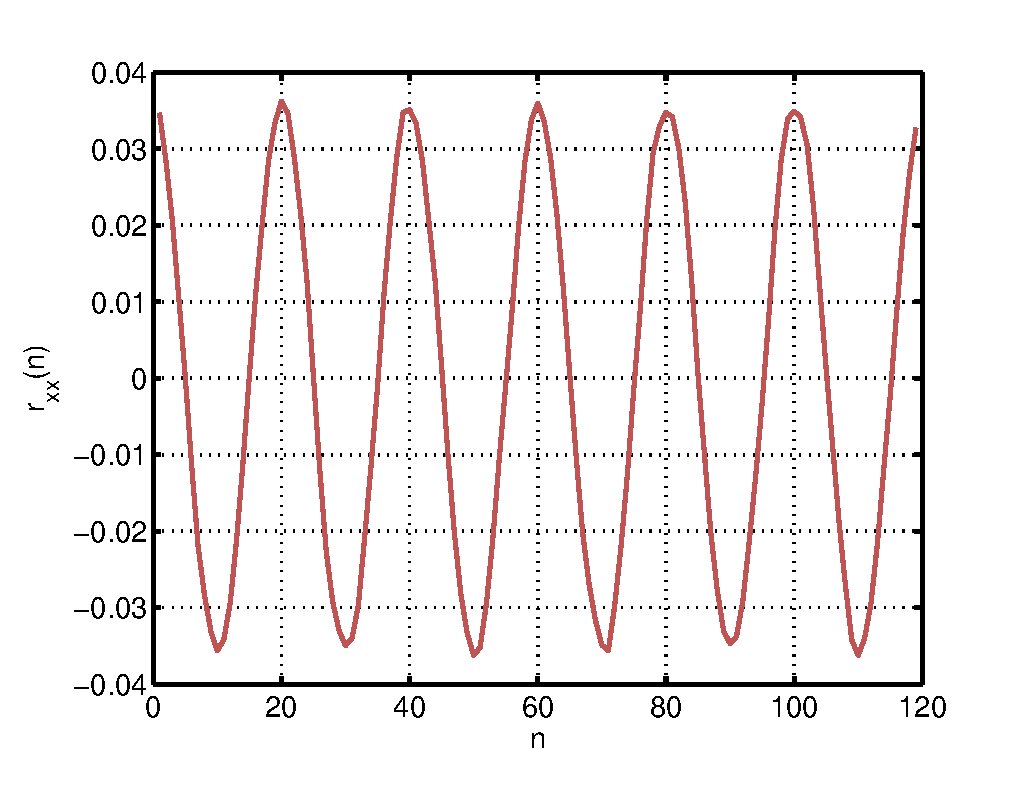
\includegraphics[width=1\linewidth]{acf_3_iter.eps}}
	\caption{Оценка АКФ на 3 итерации.}
	\label{pic:acf_3_iter}
\end{figure}

Представленный алгоритм позволяет значительно улучшить оценку АКФ. На рисунке \ref{pic:acf_3_iter} представлена оценка АКФ на 3 итерации.
Результаты работы алгоритма уточнения поступают на вход алгоритма АР. АР алгоритм позволяет точно оценить частоту гармонического сигнала.

В данной работе предложена оптимизированная версия данного алгоритма, позволяющая применять его при обработке сигнала в реальном времени.

Для снижения вычислительных затрат указанный алгоритм предлагается реализовывать с использованием процедуры БПФ. 
Введем следующие обозначения: ${x}$ – вектор входного сигнала после снятия ПСП, ${F}$ – матрица прямого преобразования Фурье, ${F^{-1}}$- матрица обратного преобразования Фурье.
Оценку АКФ на первом шаге можно получить следующим образом:

\begin{center}
\begin{equation}
	\label{eq:akf_1}
	\hat{r}_1 = F^{-1}\left[ Fx \cdot (Fx)^* \right] = F^{-1} \left[ \left| Fx \right| ^2 \right]
\end{equation}
\end{center}

Здесь знак ${(\cdot)}$  означает поэлементное перемножение векторов, ${\left| Fx \right| ^2}$ - поэлементное возведение модуля комплексного числа в квадрат, ${*}$ - означает
комплексное сопряжение.  Следуя алгоритму, изложенному в \cite{ostanin_akf} вычислим оценку АКФ от ${\hat{r}_1}$:

\begin{center}
\begin{eqnarray}
	\label{eq:akf_2}
	\hat{r}_2 & = & F^{-1}\left[ F \hat{r}_1 \cdot (F \hat{r}_1)^* \right] = \nonumber \\
		& = & F^{-1}	\left[ 
				FF^{-1} \left[
						\left| Fx \right| ^2
					\right]
						\cdot \left( FF^{-1} \left[ \left| Fx \right| ^2 \right]
					\right) ^*
			\right] = \nonumber \\
		& = & F^{-1} \left[ \left| Fx \right| ^2 \cdot \left[ \left| Fx \right| ^2 \right] ^* \right] =  \nonumber \\
		& = & F^{-1} \left[ \left| Fx \right| ^4 \right]
\end{eqnarray}
\end{center}

Рассуждая аналогично, можно показать, что уточненная оценка АКФ на K-ом шаге алгоритма, рассмотренного в \cite{ostanin_akf}
может быть получена без использования итераций с помощью выражения:

\begin{center}
\begin{equation}
	\label{eq:akf_3}
	\hat{r}_K = F^{-1}\left[ \left| Fx \right| ^{2^K} \right]
\end{equation}
\end{center}

Схематически алгоритм получения уточненной оценки АКФ на третьем шаге представлен на рисунке \ref{pic:akf_pic}.

\begin{figure}[H]
	\center\scalebox{0.8}{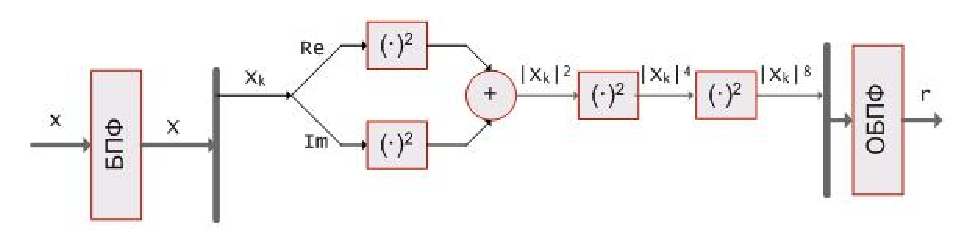
\includegraphics[width=1\linewidth]{akf_fft.eps}}
	\caption{Усовершенствованный итеративный алгоритм получения АКФ}
	\label{pic:akf_pic}
\end{figure}

%%%%%%%%%%%%%%%%%%%%%%%%%%%%%%%%%%%%%%%%%%%%%%%%%%%%%%%%%%%%%%
\subsection{Алгоритм обнаружения и оценки параметров ШПС в условиях интерференции (DMA + уточненный АР)}
\label{sec4:dma_lpc_algo}

В данной работе предлагается объединить результаты работы алгоритма DMA, рассмотренного в разделе
\ref{sec1:dma_real} и, предложенных в данной работе, усовершенствованного итеративного 
алгоритма уточнения АКФ (раздел \ref{ssec4:quadruple}) гармонического сигнала и 
подхода для оценки частоты ПСП-модулированного сигнала при помощи АР-модели (раздел \ref{ssec4:lpc_cdma_detect}).

Схематично алгоритм изображен на рисунке \ref{pic4:dma_quadruple_lpc}

\begin{figure}[H]
\center\scalebox{1}{\includegraphics[width=1\linewidth]{dma_quadruple_lpc.eps}}
	\caption{Алгоритм обнаружения и оценки параметров ШПС в условиях интерференции (DMA + уточненный АР)}
	\label{pic4:dma_quadruple_lpc}
\end{figure}

Выходом алгоритма DMA является оценка фазы ПСП. Повторно модулируя входящий сигнал ПСП с полученной
фазой, можно восстановить гармонический сигнал. Для оценки частоты данного сигнала применяется
АР-метод. Но для оценки АР-методом, требуется точная оценка АКФ, которую можно получить
с помощью усовершенствованного итеративного алгоритма вычисления АКФ.

Рекомендации по выбору задержки ${\tau}$ и детали алгоритма DMA рассмотрены в разделе
\ref{sec1:dma_real}.

Предложенный алгоритм можно описать следующим набором шагов:
\begin{itemize}
\item[Шаг 1.] Входной сигнал ${x(k)}$ умножается на задержанную копию ${x(t-\tau)}$. Так же
	на данном шаге можно производить когерентное накопление результата, для
	увеличения ОСШ.

	\begin{center}
	\begin{equation}
		%\label{}
		x_{new}(k) = \frac{C_{new}(k)}{2} \left(\cos (2\pi f \tau) - \cos \left[2 \pi f (2t - \tau)\right]\right)
	\end{equation}
	\end{center}

\item[Шаг 2.] Полученный сигнал ${x_{new}(k)}$ фильтруется ФВЧ для отсечения высокочастотной компоненты.
\item[Шаг 3.] Генерируется локальная ПСП ${C(k)}$ и умножается на задержанную копию ${C(k-\tau)}$.

	\begin{center}
	\begin{equation}
		%\label{}
		C_{new}(k) = C(k)C(k-\tau)
	\end{equation}
	\end{center}

\item[Шаг 4.] Отфильтрованный сигнал ${x_{filt}(k)}$ коррелируется с новой ПСП ${C_{new}(k)}$
	с использованием БПФ. Выход коррелятора сравнивается с заранее определенным порогом.

	\begin{center}
	\begin{equation}
		%\label{}
		x_{filt}(k) = \frac{C_{new}(k)}{2} \cos (2\pi f \tau)
	\end{equation}
	\end{center}

	\subitem{\bf{Если}}  значение оказалось больше порогового {\bf{то}},
		принимается решение о наличии сигнала. Полученное значение фазы ПСП  - ${m}$ запоминается.
		Перейти на шаг 5.
	\subitem{\bf{Иначе}} 
		Принимается решение об отсутствии сигнала.
\item[Шаг 5.] Входной сигнал ${x(k)}$ модулируется ПСП ${C(k-m)}$. В результате получаем гармонический
	сигнал ${x_{cos}(k)}$ с неизвестной частотой.
\item[Шаг 6.] Для увеличения ОСШ сигнала ${x_{cos}(k)}$ вычисляется значение уточненное значение АКФ
	по алгоритму, предложенному в разделе \ref{ssec4:quadruple}.
\item[Шаг 7.] Определяются коэффициенты АР-модели ${\hat{a_1}, \hat{a_2}}$, по формуле \ref{eq:lpc_a_estimation}. 
	Вычисляется резонансная частота ${\omega_0 = 2 \pi f}$ и определяется квадрат модуля частотного отклика АР-модели для этой частоты. 
\end{itemize}

Количество итераций требуемых для оценки частоты одного источника:
\begin{enumerate}
\item Алгоритм DMA:
	\begin{center}
	\begin{equation}
		%\label{}
		OP_{DMA} = 8NlogN + 6N
	\end{equation}
	\end{center}
	%\subitem[1] ${N}$ - умножить входной сигнал на задержанную копию;
	%\subitem[2] \textcolor{red}{фильтрация сигнала а как мне оценить это!?} ;
	%\subitem[3] ${N \log (N)}$ - преобразование Фурье ${x_{new}(k)}$;
	%\subitem[4] ${N}$ - умножить сгенерированную ПСП на задержанную копию;
	%\subitem[5] ${N \log (N)}$ - преобразование Фурье ${C_{new}(k)}$;
	%\subitem[6] ${N}$ - умножить ${X_{new}(k)}$ и ${C_{new}(k)}$;
	%\subitem[7] ${N \log (N)}$ - обратное преобразование Фурье; 
	%\subitem[8] ${N}$ - повторная модуляция входного сигнала ПСП;
\item Усовершенствованный итеративный алгоритм получения АКФ:
	\begin{center}
	\begin{equation}
		%\label{}
		OP_{ACF} = 8NlogN + (k+2)N
	\end{equation}
	\end{center}
	%\subitem[1] ${N \log (N)}$ - преобразование Фурье ${x_{cos}(k)}$;
	%\subitem[2] ${kN}$ - ${k}$ - итераций в частотной области;
	%\subitem[3] ${N \log (N)}$ - обратное преобразование Фурье;
\item Оценка параметра АР-методом:
	\begin{center}
	\begin{equation}
		%\label{}
		OP_{AR} = 
	\end{equation}
	\end{center}
\end{enumerate}

В данном алгоритме количество итераций не зависит от количества частот в области поиска,
а зависит только от количества итераций при уточнении  АКФ:
\begin{equation}
	%\label{}
	OP_{DMA_AR} =  
\end{equation}

Количество итераций требуемых для оценки частоты одного источника параллельным корррелятором:
\begin{enumerate}
	\item ${N \log (N)}$ - преобразование Фурье входного сигнала;
	\item ${N}$ - умножить сгенерированную ПСП на локальную копию гармонического сигнала;
	\item ${N \log (N)}$ - преобразование Фурье локальной копии сигнала;
	\item ${N}$ - умножение входного сигнала и локальной копии в частотном домене;
	\item ${N \log (N)}$ - обратное преобразование Фурье;
\end{enumerate}

Нужно отметить, что шаги 2-5 требуется выполнить ${g}$ раз - сколько частот требуется перебрать.
Перебор в области частоты требуется в следствии допплеровского эффекта. Например для оценки 
параметров при детектировании сигнала системы Navstar GPS требуется перебор как минимум
11 частотных ячеек для стационарного приемника.
Таким образом общее количество операций, требуемых для оценки параметров ПСП модулированного
сигнала равно:
\begin{equation}
	%\label{}
	Operations = N \log (N) + g(2N + 2N \log (N)) 
\end{equation}

%%%%%%%%%%%%%%%%%%%%%%%%%%%%%%%%%%%%%%%%%%%%%%%%%%%%%%%%%%%%%%
%\subsection{Результаты численного моделирования}
%Предложенный в \ref{sec4:dma_lpc_algo} алгоритм состоит из нескольких стадий. На первой стадии необходимо получить фазу ПСП. Для
%оценки сравнительных характеристик алгоритма DMA со стандартным подходом, рассмотрим прием сигнала с известной фазой и
%амплитудой.
%
%Из \cite{pestryakov-book} известно, что значение порога для оптимального приемника (согласованного фильтра) для данного случая выбирается
%исходя из выражения:
%\begin{center}
%\begin{equation}
%	\label{eq4:corr_thr}
%	h = \frac{N_0}{2} \ln(\Lambda_0) + \frac{E}{2}
%\end{equation}
%\end{center}
%где ${\Lambda_0=\frac{P(H_0)}{P(H_1)}}$ - отношение вероятности пропуска к вероятности ложного срабатывания.
%
%Для численного эксперимента возьмем ${\Lambda=1}$, тогда порог ${h=\frac{E}{2}}$.
%
%В виду того, что алгоритм DMA снижает отношения ОСШ, в некоторых случаях может понадобиться увеличение уровня ОСШ для
%уверенного детектирования входного сигнала. Этого, например, можно достигнуть когерентным накапливанием сигнала, но
%это приведет к возрастанию вероятности смены фазы сигнала при переходе полярности бита данных, что приведет к пропуску сигнала.
%
%Следует отметить, что выбор порога по формуле \ref{eq4:corr_thr} не является оптимальным для алгоритма DMA. Выбор оптимального
%порога для данного случая предмет отдельного исследования. Интересный способ выбора порога предложен в работах \cite{2max_article, 2max_ieee}.
%Но вывода статистических характеристик в терминах вероятности пропуска и ложного срабатывания в данных работах не произведено.

\newpage
